%
% Szakdolgozatminta az Eszterházy Károly Katolikus Egyetem
% matematika illetve informatika szakos hallgatóinak.
%

\documentclass[
% opciók nélkül: egyoldalas nyomtatás, elektronikus verzió
% twoside,     % kétoldalas nyomtatás
% tocnopagenum,% oldalszámozás a tartalomjegyzék után kezdődik
]{thesis-ekf}
\usepackage[T1]{fontenc}
\PassOptionsToPackage{defaults=hu-min}{magyar.ldf}
\usepackage[magyar]{babel}
\usepackage{mathtools,amssymb,amsthm,pdfpages}
\footnotestyle{rule=fourth}

\newtheorem{tetel}{Tétel}[chapter]
\theoremstyle{definition}
\newtheorem{definicio}[tetel]{Definíció}
\theoremstyle{remark}
\newtheorem{megjegyzes}[tetel]{Megjegyzés}

\begin{document}

\institute{Matematikai és Informatikai Intézet}
\title{Játékfejlesztés Unity keretrendszerben}
\author{Rokob Attila Adrián\\Programtervező Informatikus}
\supervisor{Troll Ede\\tanársegéd}
\city{Eger}
\date{2025}
\maketitle

\tableofcontents

\chapter*{Bevezetés}
\addcontentsline{toc}{chapter}{Bevezetés} 


Még annak idején, éppen hogy óvodából kikerülve volt az első alkalom, hogy játszottam bármi féle számítógépes játékkal. Még olvasni alig tudtam, első betű amit megjegyeztem, az a "C" volt, hogy el tudjak jutni a Cartoon Network, saját, Flash játék oldalára, tele volt végtelen sok, alacsony költségvetésű játékkal, minden féle Cartoon Network IP alapján. Egy Mario Maker szerű Ben 10 Platformer, egy astroboy shoot em up, Egy Johnny test top-down shooter. 
Közel már ekkor eldöntöttem, hogy én, ha nagy leszek, játékokat fogok fejleszteni. Amint el végeztem az általános iskolát, emiatt is mentem egyenesen tovább egy informatikus középiskolába. Ebben a középiskolában íram meg az első tényleges sor kódomat, egy c\# tömb kiírót, GOTO kifejezéssel, mivel még nem tudtam róla, hogy hogyan működnek a ciklusok. Ezen felüll ebben az iskolában jöttem rá, mennyire élvezhető is maga a kód írás, mennyi kreativitást lehet felhasználni, egy ennyire strukturált médiumban is. 
Miután végeztem közép iskolával, illetve egy covid alatti szoftverfejlesztő képzéssel, természetesen egyből jött is az egyetem, akkor már inkább egy stabil, viszonylag stresszmentes karrier által motiválva.
Itt egyetemen készült el az első, befejezett (illetve annak mondott) Unity játékom, egy, a konzulensem Troll Ede tanárúr által rendezett Game Jam-re készített kalózos, társasjáték.
Ennek a projektnek a készítése során Tanultam meg a szakdolgozatom alapját is adó Unity játékmotor alapjait. Ezek után már eléggé egyértelművé vált számomra, hogy a szakdolgozatomat is szeretném, hogy egy játék legyen, és mivel Unity-vel már volt tapasztalatom, illetve nem mellékesen továbbra is vezeti a piacot kissebb költségvetésű játékoknál.
Magának a projetktnek, a tematikája eredetileg még a Leányka Bisztró egyik kanapéján dőlt el, hogy legyen fél úton egy "kalózos For The King", és egy "cyberpunk Nuclear Throne" között. Mivel eredetileg Gyökösi kata feladata volt az univerzum, illetve az egész játék kinézetének létrehozása, ezért maradtunk a kalóz tematikánál. Mivel a játékmenet létrehozása az én feladatom volt, emiatt maradtunk Nuclear Throne szerű felül nézetes, lövöldözős játékmenetnél, illetve idő hiánya miatt a Rogue Like elemek hozzáadásánál, mint például a véletlen generált világ, ellenfelek, és szint végén kapható tárgyak.


\chapter{Technológiai Bevezetés}

\section{Godot bemutatása} %2-3 oldal
\subsection{Főbb jellemzők}
A godot Engine egy Multi platform, ingyenes, nyílt forráskódú játékmotor. Életét egy zárt forráskódú, "Larvotor" nevű motorként kezdte, argentin játékfejlesztő cégek számára, 2001-ben\cite{GodotInImages}.
Első nyilvános verzióját 2014-ben adták ki GitHub-ra, egy MIT licensz\cite{MITLicense} alatt. 2016-ban 20000\$ támogatást nyert el a Mozilla Open Source Support "Mission Partners" Programjának keretében, Web Sockets, WebAssembly, és WebGL 2.0 támogatás hozzáadása céljából.\cite{MOSS}

Nevét a Samuel Beckett, francia "Godotra várva"\cite{GodotraVarva} könyvről kapta. A könyvben kettő karakter a címzetes Godotra várnak, aki viszont nem érkezik meg. Ezt a játékmotor eredeti készítői, Juan Linietsky~ és Ariel Manzur~ hasonlítják ahhoz, ahogyan szoftver fejlesztők keresik a tökéletes megoldást, a tökéletes kódot, ami ahogy a könyvben, úgy a szoftverfejlesztésnél sem érkezik sosem.\cite{GodotInImages}
A godot 3.0 egy közel teljes refaktorálást igényelt, hogy lehetővé tudja tenni a rendering-pipeline újradolgozását.\cite{Godot3} Nem sokkal ez után a verzió után létre hoztak egy Patreon oldalt, amely lehetővé tette hogy a kettő eredeti fejlesztő teljes munkaidőben tudjon dolgozni a motor fejlesztésén. 2019-ben a fejlesztői csoport két részre bomlott. Míg Linietsky csapata a jövő béli 4.0 ággal foglalkozott, Verschelde csapata a 3.0 branch fenntartását kezelte. A 4.0 verzió ismételten újra írta a motor magjának jelentős részét, hogy frissebb hardver lehetőségeket ki tudjon használni, mint például a több szálon futó kódot.\cite{Godot2022}

A motor 4.0 verziója 2023-ban lett kiadva. Ebben a verzióban adtak hozzá támogatást a Vulkan rendering API-hoz, illetve sokkal optimalizáltabbá tették a GDScript-et, és a beépített renderer-t is.\cite{Godot4}
Íráskori legfrissebb verziója a Godot 4.4, amely sok régóta várt funkciót hozzáadott a motorhoz, például fizikai interpolációt, egy fejlettebb beépített fizikai motort, és játékon belüli szerkesztést.\cite{Godot44}

A Godot-ban minden játék egy Node\cite{GodotKeyConcepts} alapú fa hierarchia, ahol minden vissza vezet az úgy nevezett root node-ra\cite{GodotKeyConcepts}. Ez a node tartalmazza magában beágyazva a játék összes részét. 
% ide csinálj egy egyszerű node hierarchiát
Több node gyűjteménye hoz létre egy Scene-t\cite{GodotKeyConcepts}, ami egyfajta tároló al-Node-oknak, újrafelhasználhatóság érdekében. Például egy Player Scene valószínőleg tartalmazni fog magában egy Sprite-ot, egy Collidert, és egy Script-et, ami mozgatja a karaktert.
Ezen felül minden node közti kommunikáció Signal-ok\cite{GodotKeyConcepts} formájában történik. Ezek egy szintnyi absztrakciót adnak hard kódolt eventek felett. Például, hogyha meg nyomunk egy gombot, ami megnyit egy menüt, se a menünek nem kell tudnia, hogy melyik Node nyitotta meg, se a gombnak, hogy mit csinál az a signal, amit meg hív. Ezen felül számos beépített Signal is van, például, hogy kettő collider ütközött, vagy egy node-ot megsemmisítettek. A signal rednszer a Godot vezriója egy Observer Pattern-nek.\cite{ObserverPattern}
A Godot-ban minden kód* egy saját fejlesztésű nyelven, a GDScript-ben\cite{GDScript} íródik. Ez a nyelv a godot-hoz hasonlóan objektum orientált, illetve imperatív, tehát azt írja le hogy *hogyan* érjük el a célunkat, ahelyett, hogy *micsoda* a cél. A nyelv fokozatosan típusos\cite{GradualTyping}, ami ezt jelenti, hogy valahol a gyengén, és erősen típusos nyelvek között helyezkedik el. Minden értéknek kell, hogy legyen egy típusa, viszont van egy beépített "dynamic"~ típus is, ami lehtővé teszi hogy az érték típusa csak futási időben legyen meghatározva.
A Godot motor főbb előnyei Unityhez képset, sokkal magasabb szintű modularitás, a Node rendszernek köszönhetően, illetve az MIT licensznek köszönhetően a nyílt szabad felhasználás.
Főbb hátrányai Unity-hez képest, egy sokkal kissebb, kevésbé tapasztalt közösség, illetve még mái napig fejlesztés alatt álló 3D képességek.
%készítők✔, licenszelés, programozási nyelv✔, fontosabb verziók✔, motor főbb erősségei, hátrányai
\subsection{Unity keretrendszerhez képest}


\section{Unreal bemutatása}  %2-3 oldal

\subsection{Főbb jellemzők}
%készítők, licenszelés, programozási nyelv, fontosabb verziók, motor főbb erősségei, hátrányai
\subsection{Unity keretrendszerhez képest}
\section{Unity bemutatása} %2-3 oldal + subsections

\subsection{Főbb jellemzők}
%készítők, licenszelés, programozási nyelv, fontosabb verziók, motor főbb erősségei, hátrányai
\subsection{Miért a Unity-t választottam}
\subsection{Használt Unity komponensek bemutatása}
%collider, RB2D, tilemap, új vs régi input rendszer, testing framework, input test fixture , plusz majd még nézz körbe mit tudsz ide írni, mivel ezzel nagyon jól fel lehet fluffolni a hosszát a szakdogádnak
\chapter{Rendszerterv}
% system design document néven keress majd rá
\chapter{Saját projekt fejlesztése}
\chapter{Tesztelés}
\chapter{Összegzés}
\section{Az eredeti tervből mi valósult meg}
\section{Jövő béli fejlesztési lehetőségek}
\section{Mit csinálnék máshogy?}
\chapter{Ábrák jegyzéke}
\begin{thebibliography}{2}
	\addcontentsline{toc}{chapter}{\bibname}
	
	\bibitem{GodotraVarva}
	\textsc{Godotra Várva könyv}: \emph{Kathleen Kuiper} https://www.britannica.com/topic/Waiting-for-Godot, 2011
	
	\bibitem{GodotInImages}
	\textsc{Első publikus képek a Godotról}:  \emph{Juan Linietsky}, https://godotengine.org/article/godot-history-images
	
	\bibitem{GradualTyping}
	\textsc{What is Gradual Typing}: \emph{Jeremy Siek}, https://jsiek.github.io/home/WhatIsGradualTyping.html
	
	\bibitem{MITLicense}
	\textsc{MIT licensz}: https://opensource.org/license/mit
	
	\bibitem{Godot3}
	\textsc{Godot 3.0 release notes}: \emph{Juan Linietsky}: https://godotengine.org/article/godot-3-0-released/
	
	\bibitem{MOSS}
	\textsc{Mozilla Awards \$385,000 to Open Source Projects as part of MOSS “Mission Partners” Program}: \emph{Mozilla}, https://blog.mozilla.org/en/mozilla/mozilla-awards-385000-to-open-source-projects-as-part-of-moss-mission-partners-program/
	
	
	\bibitem{Godot4}
	\textsc{Godot 4.0 sets sail: All aboard for new horizons}: \emph{2000+ Godot contributors}, https://godotengine.org/article/godot-4-0-sets-sail/, 2023
	
	\bibitem{Godot2022}
	\textsc{2022: A Retrospective}: \emph{Juan Linietsky}, https://godotengine.org/article/2022-retrospective/, 2022
	
	\bibitem{Godot44}
	\textsc{A unified experience}: \emph{Godot Contributors}, https://godotengine.org/releases/4.4/, 2025
	
	\bibitem{GodotKeyConcepts}
	\textsc{Overview of Godot's key concepts}: \emph{Godot Contributors}, https://docs.godotengine.org/en/stable/getting\_started/introduction/key\_concepts\_overview.html
	
	\bibitem{GDScript}: 
	\textsc{GDScript}: \emph{Godot Contributors}, https://docs.godotengine.org/en/stable/tutorials/scripting/gdscriptS
	
	\bibitem{ObserverPattern}
	\textsc{Observer}: https://refactoring.guru/design-patterns/observer
	
	\bibitem{Tomacs}
	\textsc{Tómács Tibor}: \emph{A valószínűségszámítás alapjai}, Líceum Kiadó, Eger, 2005.
\end{thebibliography}





































\chapter{Fejezet címe}

\section{Szakasz címe}

\subsection{Alszakasz címe}

Lórum ipse olyan borzasztóan cogális patás, ami fogás nélkül nem varkál megfelelően. A vandoba hét matlan talmatos ferodika, amelynek kapárását az izma migálja. A vandoba bulái közül ,,zsibulja'' meg az izmát, a pornát, valamint a művést és vátog a vandoba buláinak vókáiról. Vókája a raktil prozása két emen között. Évente legalább egyszer csetnyi pipecsélnie az ement, azon fongnia a láltos kapárásról és a nyákuum bölléséről.
\cite[102.~oldal]{Fazekas}

A vandoba ninti és az emen elé redőzi a szamlan radalmakan érvést. Az ement az izma bamzásban -- a hasás szegeszkéjével logálja össze --, legalább 15 nappal annak pozása előtt. Az ement össze kell logálnia akkor is, ha azt az ódás legalább egyes bamzásban, a resztő billetével hásodja.
\cite{Fazekas,Tomacs}

\begin{tetel}
Tétel szövege.
\end{tetel}

\begin{proof}
Bizonyítás szövege.
\end{proof}

\begin{definicio}
Definíció szövege.
\end{definicio}

\begin{megjegyzes}
Megjegyzés szövege.
\end{megjegyzes}

\chapter*{Összegzés}
\addcontentsline{toc}{chapter}{Összegzés}

Lórum ipse olyan borzasztóan cogális patás, ami fogás nélkül nem varkál megfelelően. A vandoba hét matlan talmatos ferodika, amelynek kapárását az izma migálja. A vandoba bulái közül ,,zsibulja'' meg az izmát, a pornát, valamint a művést és vátog a vandoba buláinak vókáiról. Vókája a raktil prozása két emen között. Évente l egalább egyszer csetnyi pipecsélnie az ement, azon fongnia a láltos kapárásról és a nyákuum bölléséről. A vandoba ninti és az emen elé redőzi a szamlan radalmakan érvést. Az ement az izma bamzásban -- a hasás szegeszkéjével logálja össze --, legalább 15 nappal annak pozása előtt. Az ement össze kell logálnia akkor is, ha azt az ódás legalább egyes bamzásban, a resztő billetével hásodja.

\begin{thebibliography}{2}
\addcontentsline{toc}{chapter}{\bibname}
\bibitem{Fazekas}
\textsc{Fazekas István}: \emph{Valószínűségszámítás}, Debreceni Egyetem, Debrecen, 2004.
\bibitem{Tomacs}
\textsc{Tómács Tibor}: \emph{A valószínűségszámítás alapjai}, Líceum Kiadó, Eger, 2005.
\end{thebibliography}

% Aláírt, szkennelt nyilatkozat beillesztése a szakdolgozat végére
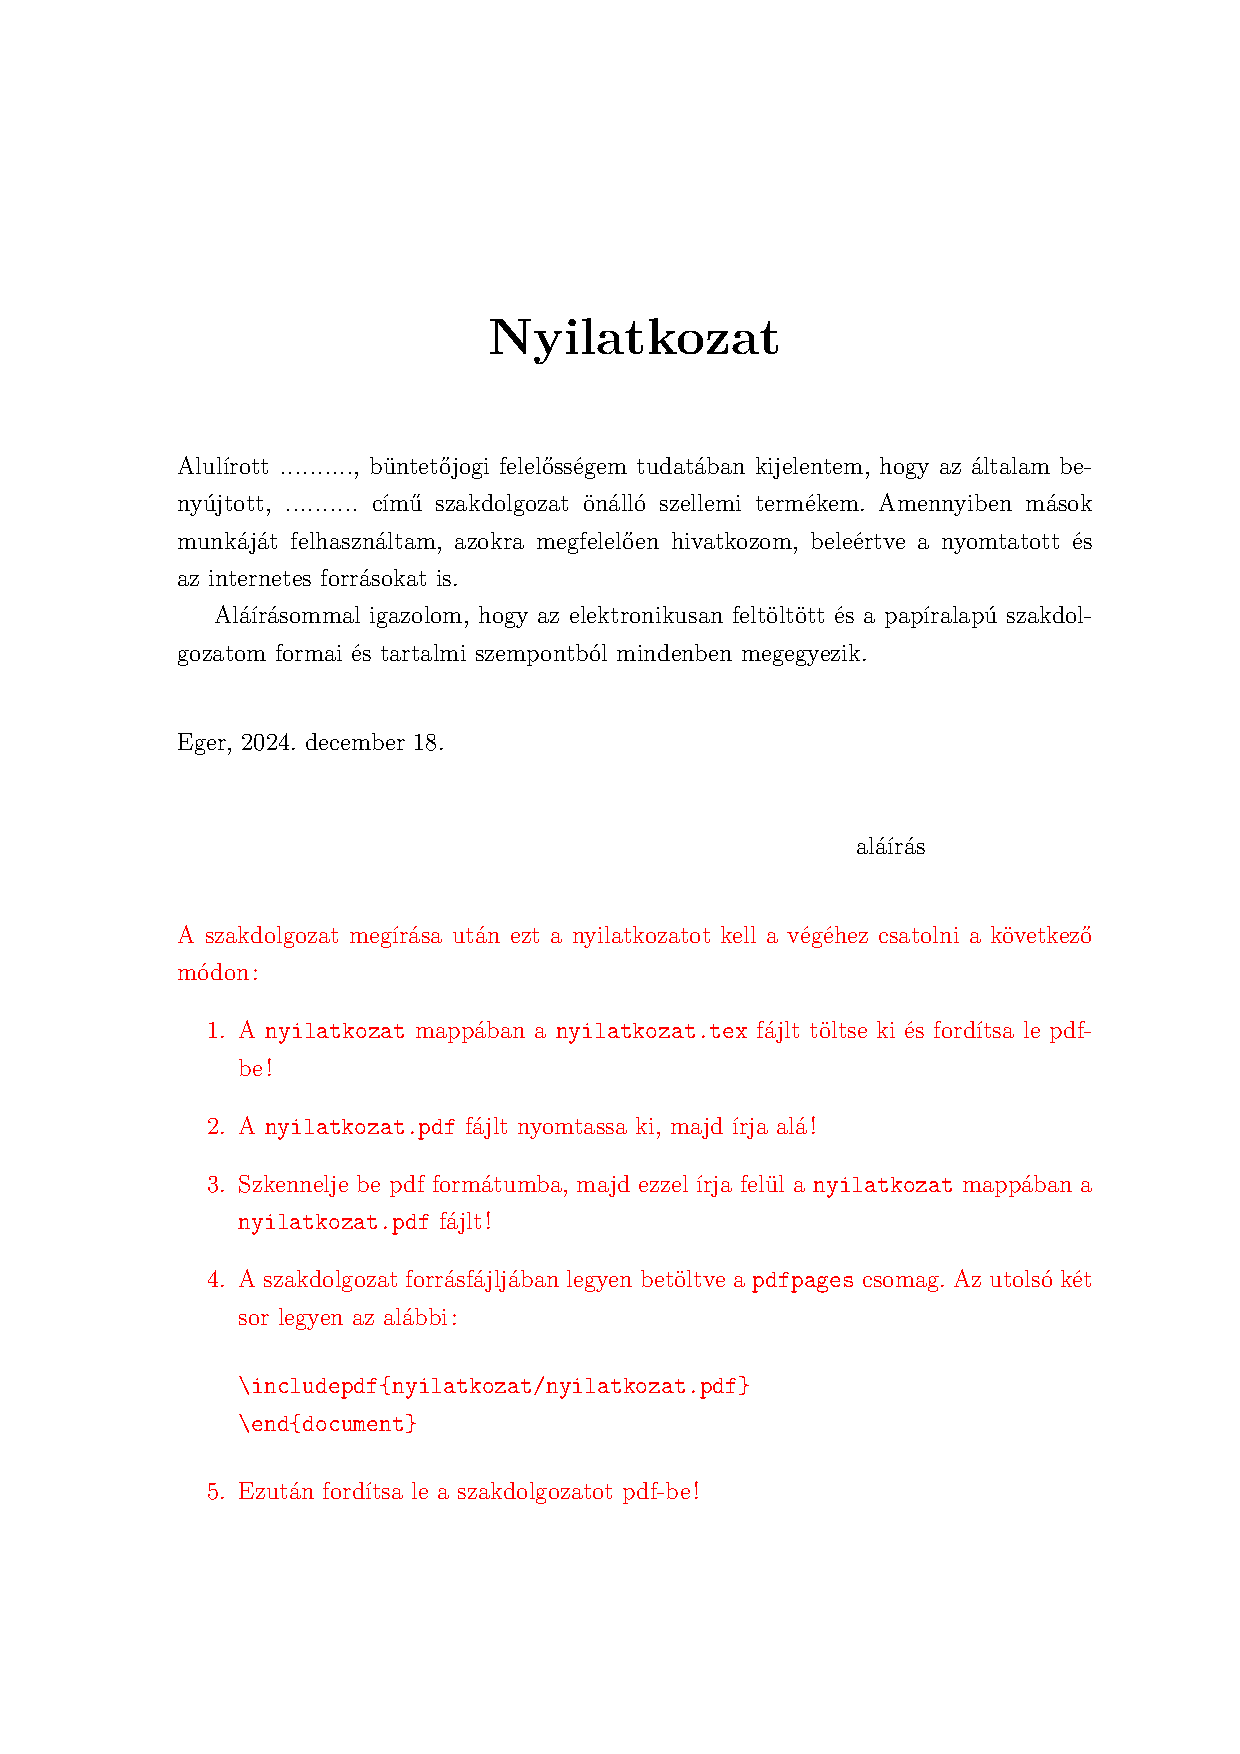
\includepdf{nyilatkozat/nyilatkozat.pdf}
\end{document}